\documentclass[12pt]{article}
\usepackage[utf8]{inputenc}
\usepackage{amsmath,amssymb}
\usepackage{float}
\usepackage{graphicx}
\usepackage[a4paper, margin=2.54cm]{geometry}
\usepackage{enumerate}
\usepackage{xcolor}
\usepackage{caption}
\usepackage{fancyhdr}
\usepackage{pgfplots}
\usepackage{enumitem}
\usepackage{tikz}
\usepackage{tikz-3dplot} % Permite coordenadas 3D
% Definir un comando para el número de pregunta en azul
\newcommand{\question}[1]{\textcolor{blue}{\textbf{#1}}}
%\usepackage[spanish]{babel}
\setlength{\headheight}{14.5pt} % Ajustar la altura del encabezado
\usetikzlibrary{3d}
\pagestyle{fancy}
\fancyhf{}
\fancyhead[L]{Taller No. 3-Teoría Electromagnética}
\fancyfoot[R]{ \thepage}
\renewcommand{\footrulewidth}{0.4pt}
\pgfplotsset{compat=1.18}
\def\a{3}      % valor de a en el eje s
\def\Emax{4}   % valor máximo de |E| en s=a
\def\b{8}      % valor de b en el eje s
\pgfmathsetmacro{\C}{\a*\Emax}        % constante para la ley 1/x
\pgfmathsetmacro{\ymax}{\Emax+1}      % tope del eje vertical
\pgfmathsetmacro{\xmax}{\b+1}         % tope del eje horizontal




\begin{document}
\begin{titlepage}
        \begin{center}
            \LARGE \textbf{Taller No. 3\\Teoría Electromagnética}
            \vfill
            \large

            Karen Alejandra Freire Rosero\\
            Sonier Andrés Ortiz Castelblanco\\
            Sarah Isabel Tejada García\\
            Santiago Alejandro Pérez Ramos
            \vfill
            \textbf{Asignatura:} Teoría Electromagnética\\
            \textbf{Profesor:} Servio Tulio Pérez Merchancano, Ph.D\\
            \vfill
            Universidad del Cauca\\
            Facultad de Ciencias Naturales, Exactas y de la Educación\\
            Departamento de Física\\
            Popayán, Cauca\\
            2025
        \end{center}
\end{titlepage}
% ----------------------------------------------Ej_Angie---------------------------------

\section*{\question{Problema 2.2} }Encuentra el campo eléctrico (magnitud y dirección) a una distancia \( z \) por encima del punto medio entre dos cargas iguales y opuestas (\( \pm q \)), separadas una distancia \( d \).

\begin{figure}[ht] 
    \centering
    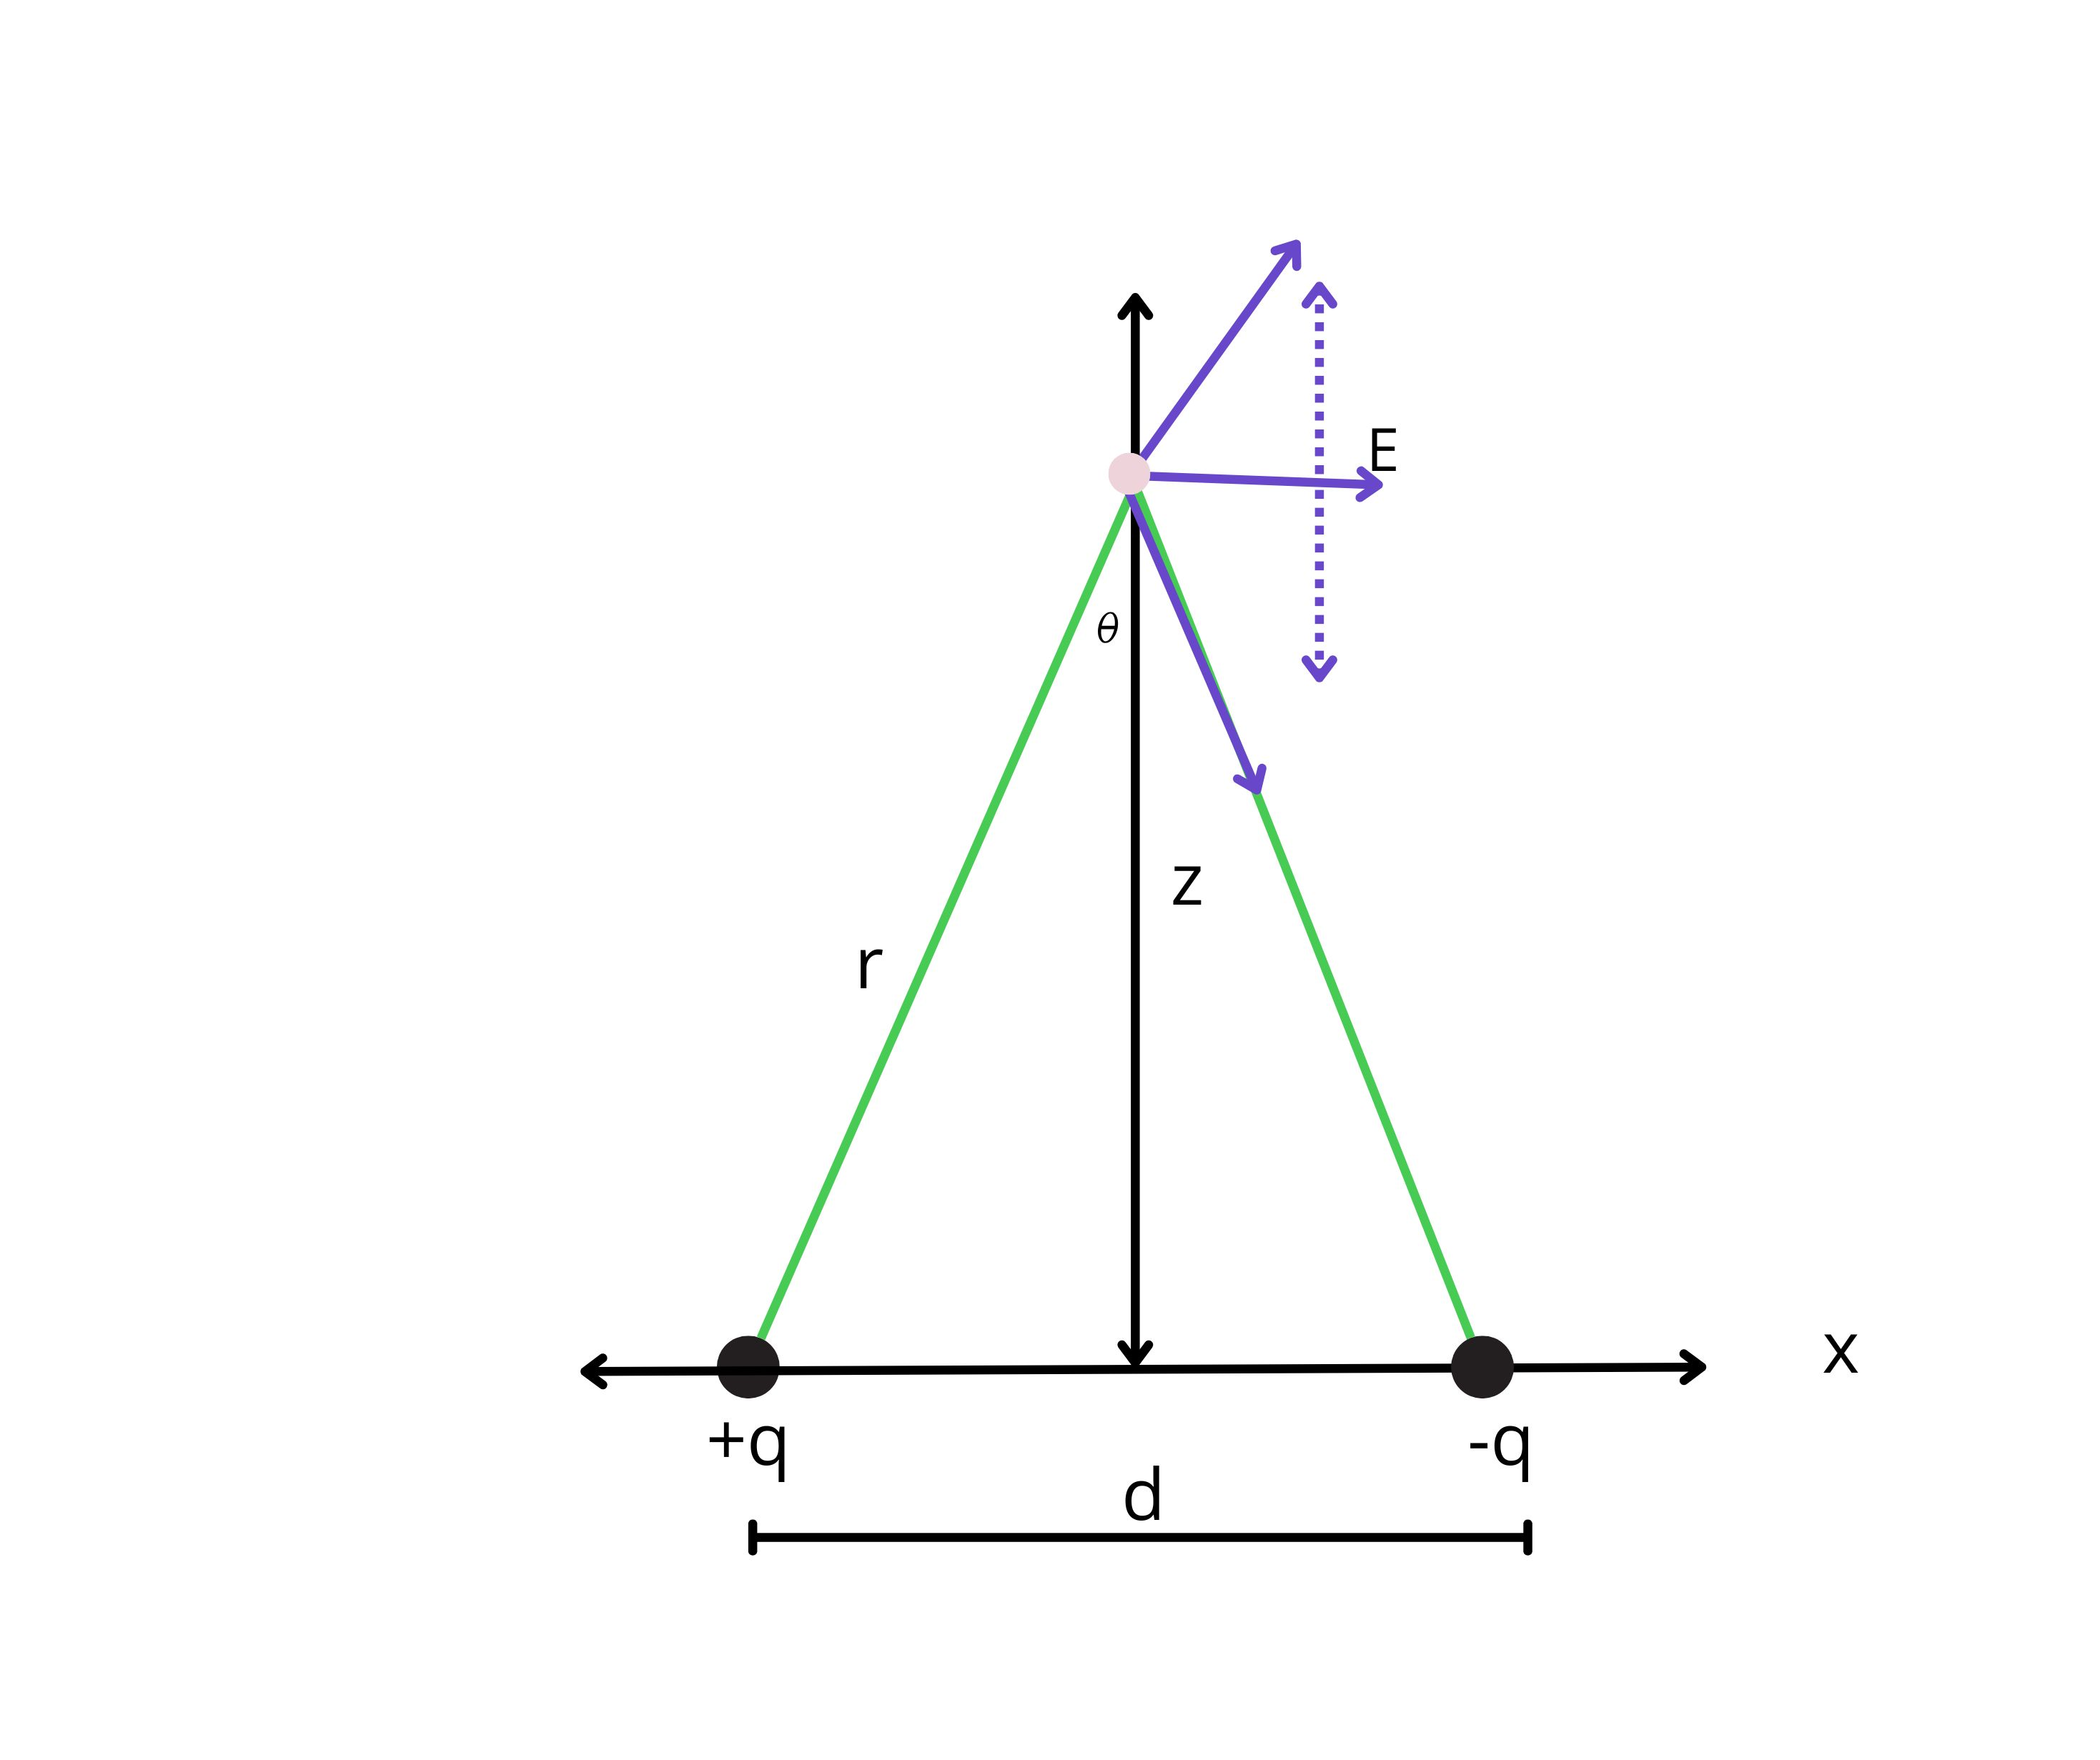
\includegraphics[width=0.7\textwidth]{imagenes/eje2.2 (1).jpg}
    \caption{Esquema del sistema}
    \label{Esquema1}
\end{figure}

\subsection*{Solución:}
Teniendo en cuenta que las componentes verticales del campo se cancelan, el campo total (Componentes en x) seria: 
\[
\mathbf{E} = \mathbf{E}_1x + \mathbf{E}_2x  
\]

\[
{E} = 2{E}_x
\]

Se tiene el siguiente triángulo con componentes del campo eléctrico:

\[
\sin \theta = \frac{E_x}{E} \quad \Rightarrow \quad E_x = E \sin \theta
\]

Entonces, como hay dos cargas que contribuyen con campos en direcciones opuestas verticalmente (que se cancelan) y horizontalmente iguales:

\[
|E_T| = 2E \sin \theta
\]

Donde:

\[
\sin \theta = \frac{d/2}{r} = \frac{d}{2r}
\]

\[
r = \sqrt{\left( \frac{d}{2} \right)^2 + z^2}
\]

\[
\sin \theta = \frac{d}{2 \sqrt{\left( \frac{d}{2} \right)^2 + z^2}}
\]

El campo eléctrico de una carga puntual \( q \) es:

\[
E = \frac{1}{4\pi \varepsilon_0} \cdot \frac{q}{r^2}
\]

Entonces:

\[
E_T = 2 \cdot \frac{1}{4\pi \varepsilon_0} \cdot \frac{q}{\left( \left( \frac{d}{2} \right)^2 + z^2 \right)} \cdot \frac{d}{2 \sqrt{\left( \frac{d}{2} \right)^2 + z^2}}
\]
Por tanto: 
\[
\boxed{
{E} = \frac{1}{4\pi\varepsilon_0} \cdot \frac{qd}{\left(z^2 + \left(\frac{d}{2}\right)^2\right)^{3/2}} \,
}
\]
\[
\boxed{
\mathbf{E} = \frac{1}{4\pi\varepsilon_0} \cdot \frac{qd}{\left(z^2 + \left(\frac{d}{2}\right)^2\right)^{3/2}} \, \hat{x}
}
\]

\section*{\question{Problema 2.4} }Encuentra el campo eléctrico a una distancia \( z \) por encima del centro de un lazo cuadrado (de lado \( a \)) que lleva una carga lineal uniforme \( \lambda \) (Figura \ref{figura2}).Pista: Usa el resultado del Ejercicio 2.2.

\begin{figure}[ht] 
    \centering
    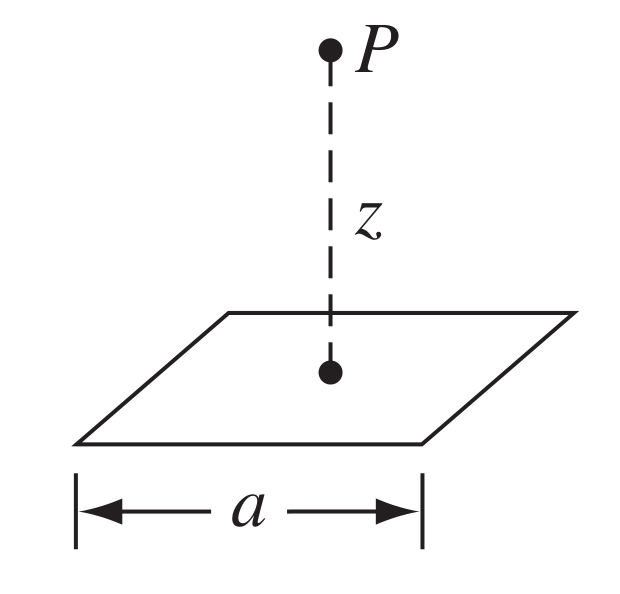
\includegraphics[width=0.3\textwidth]{imagenes/eje2.4.png} 
    \caption{Esquema del sistema}
    \label{figura2}
\end{figure}

\subsection*{Solución:}
Resultado del Ejercicio 2.2:
\[
 \mathbf{E} = \frac{1}{4\pi\varepsilon_0} \cdot \frac{2\lambda L}{z \sqrt{z^2 + L^2}} \, \hat{z}
\]
En este  caso, cada lado del cuadrado tiene longitud $a$, así que $L = \frac{a}{2}$. Además, la distancia desde el punto $P$ hasta el centro de un lado es:

\[
r = \sqrt{z^2 + \left(\frac{a}{2}\right)^2}
\]

Por tanto, el campo debido a un lado es:

\[
E_1 = \frac{1}{4\pi\varepsilon_0} \cdot \frac{\lambda a}{\sqrt{z^2 + \frac{a^2}{4}} \cdot \sqrt{z^2 + \frac{a^2}{2}}}
\]

Como hay cuatro lados, y por simetría solo contribuyen las componentes verticales, entonces:

\[
\mathbf{E} = 4 \cdot E_1 \cdot \cos\theta \cdot \hat{z}
\]

Donde: 
\[
\cos\theta = \frac{z}{\sqrt{z^2 + \frac{a^2}{4}}}
\]

Por tanto:


\[
\boxed{
\mathbf{E} = \frac{1}{4\pi\varepsilon_0} \cdot \frac{4\lambda a z}{\left(z^2 + \frac{a^2}{4}\right) \sqrt{z^2 + \frac{a^2}{2}}} \, \hat{z}
}
\]

\section*{\question{Problema 2.6} }Encuentra el campo eléctrico a una distancia \( z \) sobre el centro de un disco circular plano de radio \( R \) que tiene una densidad de carga superficial uniforme \( \sigma \). ¿Qué da la fórmula en el límite \( R \to \infty \)? También revisa el caso \( z \gg R \).

\subsection*{Solución:}
Se divide el disco en anillos concéntricos de radio \( r \) y espesor \( dr \). 

\begin{figure}[ht] 
    \centering
    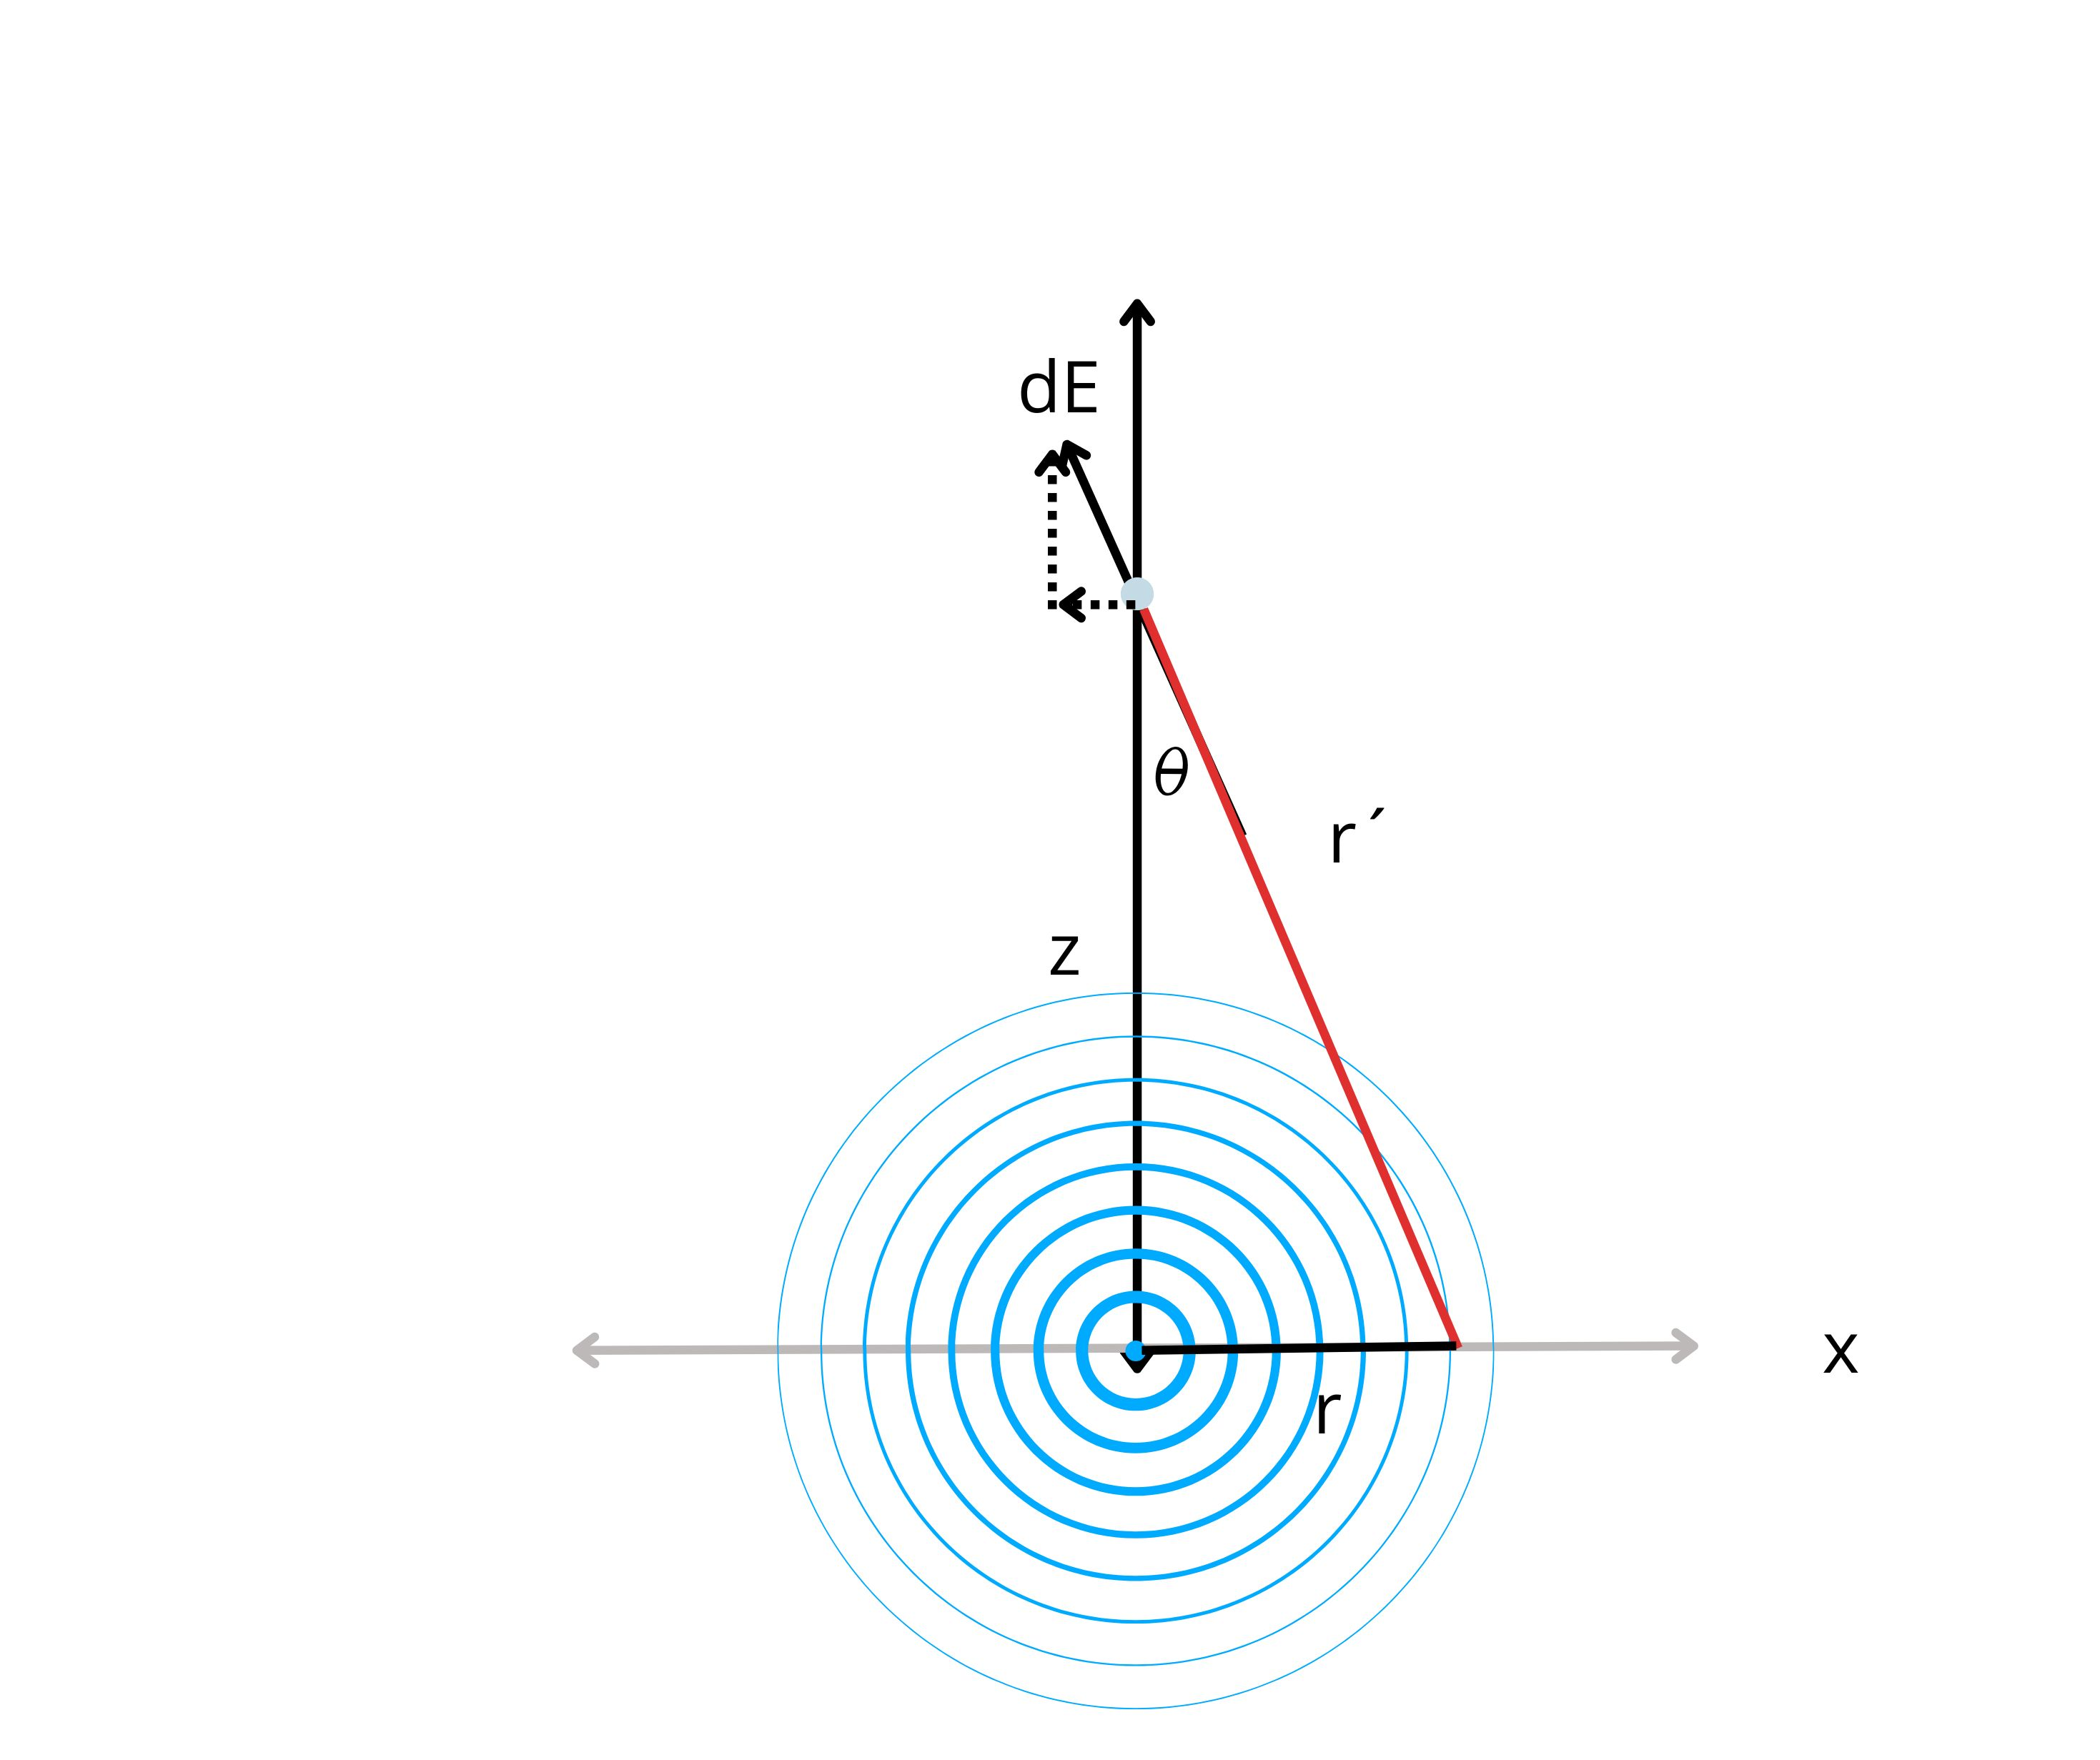
\includegraphics[width=0.5\textwidth]{imagenes/eje2.6.jpg} 
    \caption{Esquema problema 2.6}
    \label{Esquema3}
\end{figure}


La contribución al campo eléctrico en el eje \( z \), debido a esta carga \( dq \), es:

\[
d\mathbf{E} = \frac{1}{4\pi \varepsilon_0} \cdot \frac{dq}{r'^2} \cdot \hat{r}'
\]

La distancia desde el anillo hasta el punto sobre el eje \( z \) es:

\[
r' = \sqrt{r^2 + z^2}
\]

Solo la componente en \( z \) contribuye al campo, por simetría. Entonces:

\[
dE_z = \frac{1}{4\pi \varepsilon_0} \cdot \frac{dq}{r'^2} \cdot \cos\theta = \frac{1}{4\pi \varepsilon_0} \cdot \frac{dq}{r'^2} \cdot \frac{z}{\sqrt{r^2 + z^2}} = \frac{1}{4\pi \varepsilon_0} \cdot \frac{z \, dq}{(r^2 + z^2)^{3/2}}
\]

La carga en el anillo es:

\[
dq = \sigma \cdot dA = \sigma \cdot 2\pi r \, dr
\]


Se sustituye \( dq = \sigma 2\pi r \, dr \):

\[
dE_z = \frac{1}{4\pi \varepsilon_0} \cdot \frac{z \cdot \sigma \cdot 2\pi r \, dr}{(r^2 + z^2)^{3/2}} = \frac{\sigma z}{2\varepsilon_0} \cdot \frac{r \, dr}{(r^2 + z^2)^{3/2}}
\]

Para encontrar el campo eléctrico en el disco:
\[
\int_0^R dE_z = \int_0^R \frac{1}{4\pi\varepsilon_0} \cdot \frac{2\pi z \sigma \, r \, dr}{(z^2 + r^2)^{3/2}}
\]

\[
E_z = \frac{2\pi z \sigma}{4\pi \varepsilon_0} \int_0^R \frac{r \, dr}{(z^2 + r^2)^{3/2}} = \frac{\sigma z}{2\varepsilon_0} \int_0^R \frac{r \, dr}{(z^2 + r^2)^{3/2}}
\]

Resolviendo la integral:

\[
I = \int_0^R \frac{r \, dr}{(z^2 + r^2)^{3/2}}
\]

Se hace el cambio de variable:

\[
r = z \tan\theta \quad \Rightarrow \quad dr = z \sec^2 \theta \, d\theta
\]

Entonces:

\[
I = \int \frac{z \tan\theta \cdot z \sec^2 \theta \, d\theta}{\left(z^2 \tan^2\theta + z^2\right)^{3/2}}
= \int \frac{z^2 \tan\theta \sec^2 \theta \, d\theta}{z^3 (\tan^2\theta + 1)^{3/2}}
\]

\[
= \frac{z^2}{z^3} \int \frac{\tan\theta \sec^2\theta}{\sec^3\theta} \, d\theta
= \frac{1}{z} \int \frac{\tan\theta}{\sec\theta} \, d\theta
= \frac{1}{z} \int \sin\theta \, d\theta
\]

\[
= \frac{1}{z} (-\cos\theta)
\]

Volviendo a la variable original:

\[
\tan\theta = \frac{r}{z} \Rightarrow \theta = \tan^{-1}\left( \frac{r}{z} \right)
\Rightarrow \cos\theta = \frac{z}{\sqrt{z^2 + r^2}}
\]

Entonces:

\[
I = -\frac{1}{z} \left[ \frac{z}{\sqrt{z^2 + r^2}} \right]_0^R 
= -\frac{1}{\sqrt{z^2 + R^2}} + \frac{1}{z}
\]

Sustituyendo en la expresión para \( E_z \):

\[ 
\boxed{
\mathbf{E}  = \frac{\sigma z}{2 \varepsilon_0} \left( \frac{1}{z} - \frac{1}{\sqrt{z^2 + R^2}} \right) \hat{z}
}
\]


\subsection*{ Cuando \( R \to \infty \) }

Cuando \( R \to \infty \), la raíz \( \sqrt{z^2 + R^2}  \to \infty  \), así que:

\[
\frac{1}{\sqrt{z^2 + R^2}} \to 0
\]

Entonces el campo se vuelve:

\[
E = \frac{\sigma z}{2 \varepsilon_0} \left( \frac{1}{z} - 0 \right) 
\]
\[
\boxed {
\mathbf{E}  =\frac{\sigma}{2\varepsilon_0} \hat{z}
}
\]



\subsection*{Cuando \( z \gg R \) }

Cuando estamos muy lejos del disco, es decir, \( z \gg R \), podemos hacer una expansión de Taylor:

\[
\sqrt{z^2 + R^2} \approx z \left(1 + \frac{R^2}{2z^2}\right)
\Rightarrow \frac{1}{\sqrt{z^2 + R^2}} \approx \frac{1}{z} \left(1 - \frac{R^2}{2z^2}\right)
\]

Entonces el campo se aproxima a:

\[
E \approx \frac{\sigma z}{2 \varepsilon_0} \left( \frac{1}{z} - \frac{1}{z} \left(1 - \frac{R^2}{2z^2} \right) \right)
= \frac{\sigma z}{2 \varepsilon_0} \left( \frac{R^2}{2z^3} \right)
\]
\[ 
\boxed{
\mathbf{E}  = \frac{\sigma R^2}{4\varepsilon_0 z^2}\, \hat{z}
}
\]



%----------------------------------------------Ej_Angie----------------------------------
%----------------------------------------------Ej_Elizabeth---------------------------------


\section*{\question{ Problema 2.8}}  

Usando el resultado del Problema 2.7, se desea encontrar el campo eléctrico dentro y fuera de una esfera sólida de radio \( R \), que posee una densidad de carga volumétrica uniforme \( \rho \). Expresa la solución en términos de la carga total \( q \) y dibuja una gráfica cualitativa del valor absoluto del campo eléctrico \( |\mathbf{E}| \) en función de la distancia desde el centro.

\vspace{0.3cm}
La carga total de la esfera se puede expresar como:
\[
q = \rho \cdot \frac{4}{3} \pi R^3
\]

\subsection*{Solución:}

\subsection*{Campo eléctrico dentro de la esfera \((r < R)\)}

Ahora bien. aplicamos la ley de Gauss tomando una superficie esférica de radio \( r < R \). La carga encerrada dentro de esta superficie es:
\[
q_{\text{int}} = \rho \cdot \frac{4}{3} \pi r^3
\]

Aplicando la ley de Gauss tenemos que:
\[
E(r) \cdot 4\pi r^2 = \frac{q_{\text{int}}}{\varepsilon_0} = \frac{\rho \cdot \frac{4}{3} \pi r^3}{\varepsilon_0}
\]

Resolviendo para \( E(r) \):
\[
E(r) = \frac{\rho}{3 \varepsilon_0} r
\]

Sustituyendo \( \rho \) en términos de \( q \):
\[
\rho = \frac{3q}{4\pi R^3} \quad \Rightarrow \quad E(r) = \frac{q}{4\pi \varepsilon_0 R^3} r
\]

\subsection*{Campo eléctrico fuera de la esfera \((r \geq R)\)}

En este caso, toda la carga \( q \) está encerrada por la superficie gaussiana, por lo tanto:

\[
E(r) \cdot 4\pi r^2 = \frac{q}{\varepsilon_0}
\quad \Rightarrow \quad
E(r) = \frac{1}{4\pi \varepsilon_0} \cdot \frac{q}{r^2}
\]

A continuación se obtiene la grafica;
\begin{figure}[H]
    \centering
    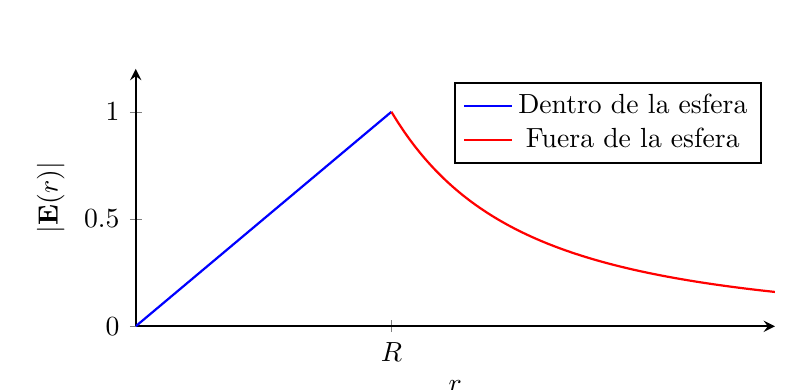
\begin{tikzpicture}
        \begin{axis}[
            axis lines = left,
            xlabel = $r$,
            ylabel = $|\mathbf{E}(r)|$,
            ymin=0, ymax=1.2,
            xmin=0, xmax=2.5,
            xtick={1},
            xticklabels={$R$},
            domain=0:2.5,
            samples=200,
            smooth,
            thick,
            width=0.8\textwidth,
            height=0.4\textwidth,
            legend style={at={(0.98,0.95)},anchor=north east}
        ]
        % Campo dentro de la esfera: E = k*r (hasta r=1)
        \addplot[blue, domain=0:1] {x};
        % Campo fuera de la esfera: E = 1/x^2 (desde r=1 en adelante)
        \addplot[red, domain=1:2.5] {1/x^2};

        \legend{Dentro de la esfera,Fuera de la esfera}
        \end{axis}
    \end{tikzpicture}
    \caption{Gráfica cualitativa de \( |\mathbf{E}(r)| \) vs. \( r \). Se normalizó el valor máximo en \( r = R \).}
\end{figure}
La gráfica de \( |\mathbf{E}(r)| \) como función de la distancia desde el centro de una esfera cargada uniformemente muestra un comportamiento característico de los campos generados por distribuciones esféricas de carga. En el interior de la esfera (\( r < R \)), el campo eléctrico crece linealmente con la distancia al centro, lo que refleja que solo la carga encerrada dentro del radio \( r \) contribuye al campo en ese punto (según la ley de Gauss). En cambio, fuera de la esfera (\( r > R \)), el campo disminuye con el cuadrado de la distancia, comportándose como si toda la carga estuviera concentrada en un punto en el centro de la esfera. Este resultado es consistente con el campo de un punto cargado, confirmando la simetría y naturaleza del campo eléctrico en distribuciones esféricas uniformes.

\section*{\question{Problema 2.10}}

Una carga puntual \( q \) se encuentra en la esquina trasera de un cubo, como se muestra en la Figura \ref{fig:figura217}. Se desea encontrar el flujo del campo eléctrico \( \mathbf{E} \) a través de la cara sombreada del cubo.


\begin{figure}[ht]
    \begin{center}
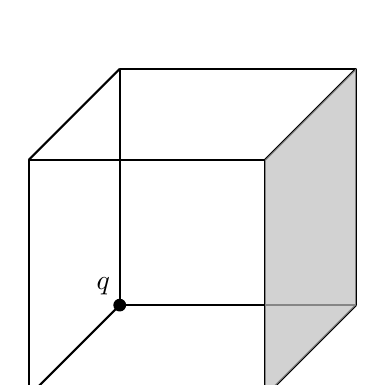
\begin{tikzpicture}[scale=3, line join=round]

  % Draw cube edges
  \draw[thick] (0,0,0) -- (1,0,0) -- (1,1,0) -- (0,1,0) -- cycle; % bottom square
  \draw[thick] (0,0,1) -- (1,0,1) -- (1,1,1) -- (0,1,1) -- cycle; % top square
  \draw[thick] (0,0,0) -- (0,0,1);
  \draw[thick] (1,0,0) -- (1,0,1);
  \draw[thick] (1,1,0) -- (1,1,1);
  \draw[thick] (0,1,0) -- (0,1,1);

  % Shade the desired face
  \fill[gray!50,opacity=0.7] (1,0,0) -- (1,1,0) -- (1,1,1) -- (1,0,1) -- cycle;

  % Place charge qabove
  \filldraw[black] (0,0,0) circle (0.7pt) node[above left] {$q$};

\end{tikzpicture}
\end{center}
\caption{Esquema de la carga ubicada la esquina del Cubo.}
\label{fig:figura217}
\end{figure}


\bigskip
\subsection*{Solución:}

Según la Ley de Gauss, el flujo eléctrico total a través de una superficie cerrada que encierra completamente una carga \( q \) es:

\[
\Phi_E = \frac{q}{\varepsilon_0}
\]

En este caso, la carga se encuentra ubicada en una esquina del cubo. En tres dimensiones, una esquina de un cubo es compartida por ocho cubos idénticos. Por lo tanto, la carga \( q \) se distribuiría entre ocho cubos si quisiéramos encerrar completamente la carga.

\[
\Phi_{\text{cubo}} = \frac{q}{8\varepsilon_0}
\]

Ahora bien, este flujo se distribuye entre las tres caras del cubo que están orientadas hacia afuera desde la esquina opuesta a la carga (ya que las tres caras adyacentes a la carga no reciben flujo saliente). Debido a la simetría del cubo, estas tres caras reciben cantidades iguales de flujo. Entonces, el flujo a través de una de estas caras (incluyendo la sombreada en la figura) es:

\[
\boxed{\Phi = \frac{q}{24\varepsilon_0}}
\]

\section*{\question{ Problema 2.12}} 
 Utiliza la Ley de Gauss para encontrar el campo eléctrico dentro de una esfera sólida uniformemente cargada con densidad de carga \( \rho \). Compara tu respuesta con el Problema 2.8.


\subsection*{Solución}

Usamos la Ley de Gauss para encontrar el campo eléctrico dentro de una esfera cargada de radio \( R \), con densidad de carga volumétrica constante \( \rho \). Consideramos una \textbf{superficie gaussiana} esférica de radio \( r < R \), concéntrica con la esfera cargada.

\subsection*{Ley de Gauss}

La Ley de Gauss establece:

\[
\oint \mathbf{E} \cdot d\mathbf{A} = \frac{q_{\text{int}}}{\varepsilon_0}
\]

Por simetría, el campo eléctrico es radial y de magnitud constante sobre la superficie gaussiana. Entonces:

\[
E(r) \cdot 4\pi r^2 = \frac{q_{\text{int}}}{\varepsilon_0}
\]

La carga encerrada dentro de la superficie gaussiana de radio \( r \) es:

\[
q_{\text{int}} = \rho \cdot \frac{4}{3} \pi r^3
\]

Sustituyendo en la ecuación de Gauss:

\[
E(r) \cdot 4\pi r^2 = \frac{\rho \cdot \frac{4}{3} \pi r^3}{\varepsilon_0}
\]

\[
E(r) = \frac{\rho r}{3 \varepsilon_0}
\]

Finalmente el campo eléctrico dentro de una esfera sólidamente cargada con densidad \( \rho \) es:

\[
\boxed{E(r) = \frac{\rho r}{3 \varepsilon_0}, \quad \text{para } r < R}
\]

\subsubsection*{Comparación }

En el interior de la esfera el campo crece linealmente con \( r \), mientras que fuera de la esfera decrece como \( 1/r^2 \), tal como se obtuvo en el problema 2.8.


%----------------------------------------------Ej_Elizabeth---------------------------------
%----------------------------------------------Ej_Michel---------------------------------


\section*{\textcolor{blue}{Problema 2.14}}

Encuentra el campo eléctrico dentro de una esfera que tiene una densidad de carga que es proporcional a la distancia desde el origen \(\rho = kr\), para alguna constante k.
\textit{[Pista: Esta densidad de carga no es uniforme, y debes integrar para obtener la carga encerrada.]}


\section*{Solución}

Usando la Ley de Gauss \[\oint_S \mathbf{E} \cdot d\mathbf{a} = \frac{Q_{\text{enc}}}{\varepsilon_0}
\]
\[
\textbf{E}(4\pi r^2) = \frac{Q_{\text{enc}}}{\varepsilon_0}
\]
La carga encerrada por la superficie gaussiana es:
\[
Q_{\text{enc}} = \int_V \rho \, dV \quad 
\]
\[
\text{siendo} \quad dV = r'^2 \sin\theta \, dr' \, d\theta \, d\phi
\quad \text{y} \quad \rho(r) = \kappa r'
\]

\[
Q_{\text{enc}} = \int_0^{2\pi} \int_0^{\pi} \int_0^r (\kappa r') \cdot (r'^2 \sin\theta \, dr' \, d\theta \, d\phi )
= \kappa \int_0^{2\pi} d\phi \int_0^{\pi} \sin\theta \, d\theta \int_0^r r'^3 \, dr'
\]

\[
= \kappa (2\pi)(-\cos\theta)\Big|_0^{\pi} \cdot \frac{r'^4}{4} \Big|_0^{r}
= \frac{4\pi \kappa r^4}{4}
\]

\[
Q_{\text{enc}} = \pi \kappa r^4
\]
Finalmente, reemplazando en la expresión del campo eléctrico
\[
\mathbf{E}  
= \frac{Q_{\text{enc}}}{(4\pi r^2)\varepsilon_0} 
= \frac{\pi \kappa r^4}{4\pi r^2 \varepsilon_0}
= \frac{\kappa r^2}{4\varepsilon_0} \, \hat{r}
\]

\[
\boxed{\mathbf{E} = \frac{\kappa r^2}{4\varepsilon_0} \, \hat{r}}
\]


\section*{\textcolor{blue}{Problema 2.16}}


Un cable coaxial largo (Fig.\ref{fig:figura226}) tiene una densidad de carga volumétrica uniforme \(\rho \) en el cilindro interior (radio a), y una densidad de carga superficial uniforme sobre el cilindro exterior (radio b). Esta carga superficial es negativa y tiene justo la magnitud adecuada para que el cable en su totalidad sea eléctricamente neutro.
Encuentra el campo eléctrico en cada una de las tres regiones:

\begin{enumerate}[label=(\roman*)]
    \item Dentro del cilindro interior \((s < a)\),
    \item Entre los cilindros \((a < s < b)\),
    \item Fuera del cable \((s > b)\).
\end{enumerate}
Grafica \( |E| \) como función de \( s \).

\begin{figure}[ht]
    \centering
    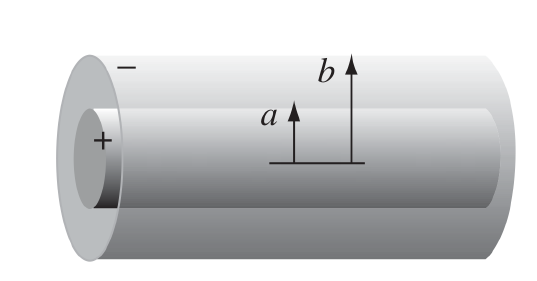
\includegraphics[width=0.5\linewidth]{imagenes/5_IMG.png}
    \caption{Esquema del cable coaxial.}
    \label{fig:figura226}
\end{figure}

\section*{Solución}

\subsubsection*{(i) Dentro del cilindro interior \((s < a)\),}

\begin{figure}[H]
    \begin{center}
        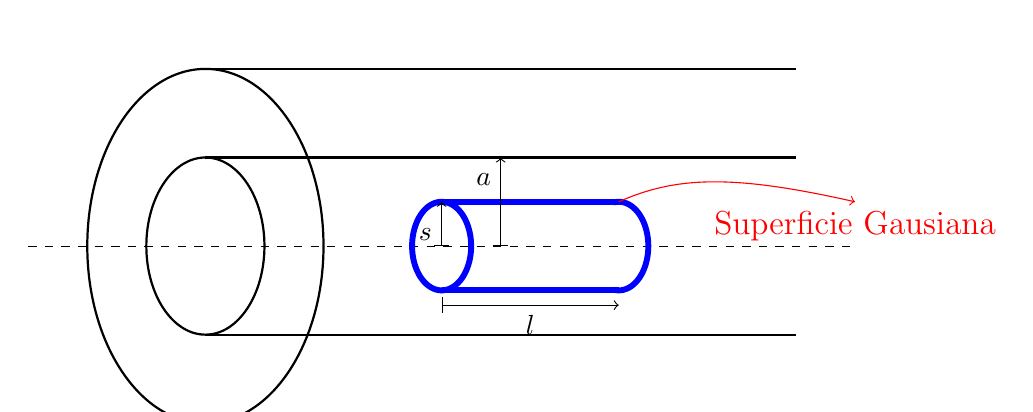
\begin{tikzpicture}[scale=0.75]
    % Outer cylinder (radius a)
    \draw[thick] (0,0) ellipse (2 and 3);
    \draw[thick] (0,0) ellipse (1 and 1.5);
    \draw[thick] (0,3) -- (10,3);
    \draw[thick] (0,1.5) -- (10,1.5);
    \draw[thick] (0,-1.5) -- (10,-1.5);
    \draw[thick] (0,-3) -- (10,-3);

    \draw[dashed](-3,0) -- (11,0);
    % cilindro de la parte interior 
    \draw[thick,blue ,domain = 0:360,samples=100, variable=\t,line width=0.75mm] 
    plot ({0.5*cos(\t)+4}, {0.75*sin(\t)});
    
    \draw[thick,blue,domain= 100:-100, samples=100, variable=\t,line width=0.75mm] 
    plot ({0.5*cos(\t)+7}, {0.75*sin(\t)});

    \draw[thick,line width=0.75mm,blue] (4,0.75) -- (7,0.75);
    \draw[thick,line width=0.75mm,blue] (4,-0.75) -- (7,-0.75);

\draw[|->] (4,-1) -- (7,-1) node[midway,below] {$l$};
    \draw[|->,dash pattern=on 2pt off 0pt] (4,0) -- (4,0.75) node[near start,left] {$s$};
    
    \draw[|->,dash pattern=on 2pt off 0pt] (5,0) -- (5,1.5) node[near end,left] {$a$};

    \draw[->,red] (7,0.75) .. controls (8,1.2) and (9,1.2) .. (11,0.75) node[below,font = \large] {Superficie Gausiana};
\end{tikzpicture}
    \end{center}
    \caption*{Superficie gaussiana \((s < a)\)\label{fig:sample}}
\end{figure}


Aplicando la Ley de Gauss
\[
\oint_S \mathbf{E} \cdot d\mathbf{a} = \frac{Q_{\text{enc}}}{\varepsilon_0}
\]

\[
\textbf{E}(2\pi s \ell) = \frac{Q_{\text{enc}}}{\varepsilon_0}
\]
La carga encerrada por la superficie gaussiana es:
\[
Q_{\text{enc}} = \int_V \rho \, dV \quad \text{donde} \quad dV = s'  ds'  d\phi  dz
\]

\[
Q_{\text{enc}} = \rho \int_0^{l} dz \int_0^{2\pi} d\phi \int_0^s s' \, ds'
= \rho \ell (2\pi) \left[ \frac{s'^2}{2} \right]_0^s
\]

\[
Q_{\text{enc}} = \pi \rho s^2 \ell
\]
Finalmente, reemplazando en la expresión del campo eléctrico
\[
\mathbf{E}= \frac{\pi \rho s^2 \ell}{ \varepsilon_0} \cdot \frac{1}{2\pi s \ell}
\]

\[
\boxed{\quad 
\textbf{E} =  \frac{\rho s}{2\varepsilon_0} \, \hat{s}
}\]

\subsubsection*{(ii) Campo eléctrico entre los cilindros \( a < s < b \)}



\begin{figure}[H]
    \centering
    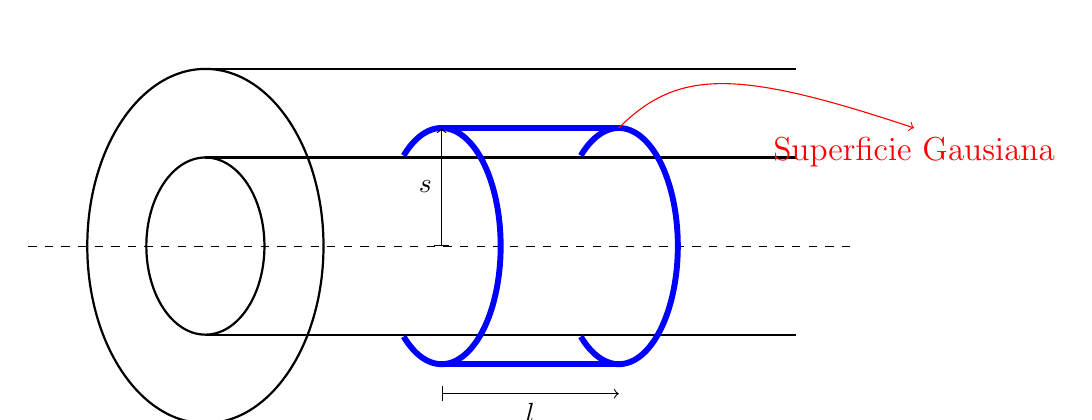
\begin{tikzpicture}[scale = 0.75]
    % Outer cylinder (radius a)
    \draw[thick] (0,0) ellipse (2 and 3);
    \draw[thick] (0,0) ellipse (1 and 1.5);
    \draw[thick] (0,3) -- (10,3);
    \draw[thick] (0,1.5) -- (10,1.5);
    \draw[thick] (0,-1.5) -- (10,-1.5);
    \draw[thick] (0,-3) -- (10,-3);

    \draw[dashed](-3,0) -- (11,0);
    % cilindro de la parte interior 
    \draw[thick,blue, domain=130:-130, samples=100, variable=\t,line width=0.75mm] 
    plot ({1*cos(\t)+4}, {2*sin(\t)});
    
    \draw[thick,blue, domain=130:-130, samples=100, variable=\t,line width=0.75mm] 
    plot ({1*cos(\t)+7}, {2*sin(\t)});

    \draw[thick,line width=0.75mm,blue] (4,2) -- (7,2);
    \draw[thick,line width=0.75mm,blue] (4,-2) -- (7,-2);
    \draw[|->] (4,-2.5) -- (7,-2.5) node[midway,below] {$l$};
    \draw[|->,dash pattern=on 2pt off 0pt] (4,0) -- (4,2) node[midway,left] {$s$};

    \draw[->,red] (7,2) .. controls (8,3) and (9,3) .. (12,2) node[below,font = \large] {Superficie Gausiana};
\end{tikzpicture}
    \caption*{Superficie gaussiana \( a < s < b \)\label{fig:sample2}}
\end{figure}

Aplicando la Ley de Gauss
\[
\oint_S \mathbf{E} \cdot d\mathbf{a} = \frac{Q_{\text{enc}}}{\varepsilon_0}
\]
\[
\textbf{E} (2\pi s \ell) = \frac{Q_{\text{enc}}}{\varepsilon_0}
\]
La carga encerrada por la superficie gaussiana es:
\[
Q_{\text{enc}} = \int_V \rho \, dV \quad \text{con} \quad dV = r \, dr d\phi dz 
\]

\[
Q_{\text{enc}} = \rho \int_0^{\ell} dz \int_0^{2\pi} d\phi \int_0^a r \, dr 
= \rho \cdot \ell \cdot (2\pi) \left[ \frac{r^2}{2} \right]_0^a 
\]
\[
Q_{\text{enc}} = \pi \rho \ell a^2
\]
Finalmente, reemplazando en la expresión del campo eléctrico
\[
\textbf{E} = \frac{1}{\varepsilon_0} \cdot \frac{(\pi \rho \ell a^2)}{(2\pi s \ell)} 
= \frac{1}{\varepsilon_0} \cdot \frac{\rho a^2}{2s} 
\quad 
\]

\[
\boxed{\quad 
\textbf{E} = \frac{\rho a^2}{2\varepsilon_0 s} \, \hat{s}
}\]

\subsubsection*{(iii) Fuera del cable \( s > b \)}



\begin{figure}[H]
    \centering
    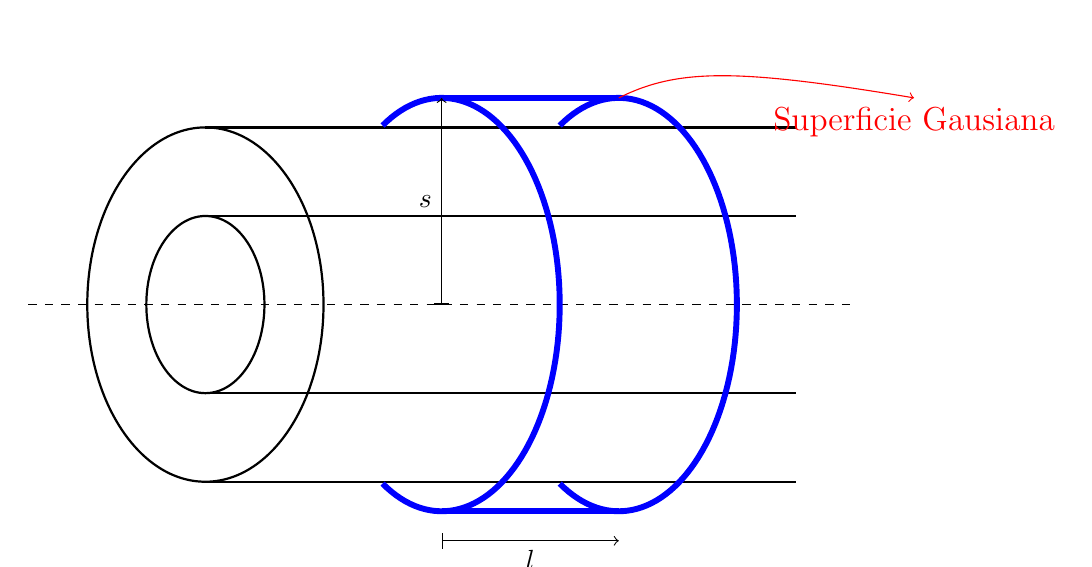
\begin{tikzpicture}[scale = 0.75]
    % Outer cylinder (radius a)
    \draw[thick] (0,0) ellipse (2 and 3);
    \draw[thick] (0,0) ellipse (1 and 1.5);
    \draw[thick] (0,3) -- (10,3);
    \draw[thick] (0,1.5) -- (10,1.5);
    \draw[thick] (0,-1.5) -- (10,-1.5);
    \draw[thick] (0,-3) -- (10,-3);

    
    \draw[dashed](-3,0) -- (11,0);
    % cilindro de la parte interior  
    \draw[thick,blue, domain=120:-120, samples=100, variable=\t, line width=0.75mm] 
      plot ({2*cos(\t)+4}, {3.5*sin(\t)});
    
    \draw[thick,blue, domain=120:-120, samples=100, variable=\t, line width=0.75mm] 
      plot ({2*cos(\t)+7}, {3.5*sin(\t)});

    \draw[thick,blue, line width=0.75mm] (4,3.5) -- (7,3.5);
    \draw[thick,blue, line width=0.75mm] (4,-3.5) -- (7,-3.5);

    \draw[|->] (4,-4) -- (7,-4) node[midway,below] {$l$};
    \draw[|->,dash pattern=on 2pt off 0pt] (4,0) -- (4,3.5) node[midway,left] {$s$};

    \draw[->,red] (7,3.5) .. controls (8,4) and (9,4) .. (12,3.5) node[below,font=\large] {Superficie Gausiana};
\end{tikzpicture}
    \caption*{Superficie gaussiana \(  s > b \)\label{fig:sample}}
\end{figure}

\[
\oint_S \mathbf{E} \cdot d\mathbf{a} = \frac{Q_{\text{enc}}}{\varepsilon_0}
\]

\[
\textbf{E} (2\pi s \ell) = \frac{Q_{\text{enc}}}{\varepsilon_0}\quad
\]
El campo fuera del cable es nulo, ya que el sistema es neutro y la simetría asegura que los campos de las cargas opuestas se cancelan fuera del cable.
\[
\boxed{\textbf{E} = 0}
\]

\subsubsection*{Gráfica \( |E| \) como función de \( s \).}

\begin{figure}[H]
  \centering
  \begin{tikzpicture}[>=latex, thick]
    % Ejes
    \draw[->] (0,0) -- (\xmax,0) node[right] {$s$};
    \draw[->] (0,0) -- (0,\ymax) node[above] {$|E|$};

    % Coordenadas clave
    \coordinate (O) at (0,0);
    \coordinate (A) at (\a,\Emax);
    % Punto B = (b, C/b) calculado automáticamente
    \coordinate (B) at (\b,{ \C/\b });

    % Fase 1: ascendente lineal (azul)
    \draw[blue] (O) -- (A);

    % Fase 2: decrecimiento 1/x (rojo)
    \draw[red,domain=\a:\b,variable=\x,samples=100]
      plot (\x,{ \C/\x });

    % Fase 3: colapso vertical (verde)
    \draw[green!60!black] (B) -- (\b,0);

    % Líneas auxiliares y etiquetas
    \draw[dashed] (A) -- (\a,0) node[below] {$a$};
    \node[below] at (\b,0) {$b$};
  \end{tikzpicture}
  \caption{Gráfica esquemática de \(|\mathbf{E} |\) vs.\ \(s\).}
  \label{fig:EvsS}
\end{figure}


\section*{\textcolor{blue}{Problema 2.18}}
Dos esferas, cada una de radio R y que llevan densidades de carga volumétrica uniformes \(+ \rho\)  y \( -\rho\), respectivamente, se colocan de forma que se superponen parcialmente (Fig. \ref{fig:figura2.28}).

\begin{figure}[ht]
    \centering
    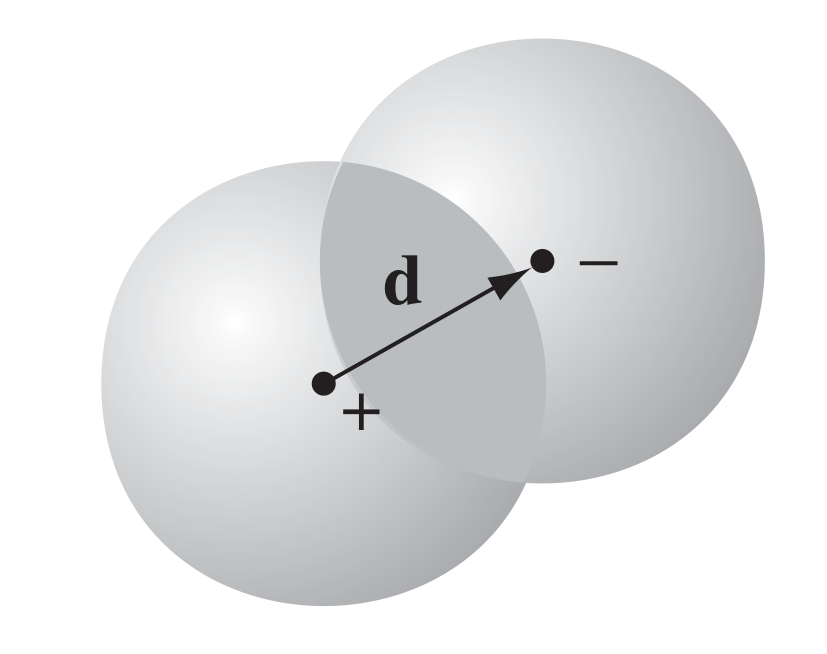
\includegraphics[width=0.4\linewidth]{imagenes/6_IMG.png}
    \caption{Esquema del problema 2.18}
    \label{fig:figura2.28}
\end{figure}

Llama al vector desde el centro positivo hacia el centro negativo d.
Demuestra que el campo en la región de superposición es constante, y encuentra su valor.
\textit{[Pista: Usa la respuesta del Problema 2.12.]}
\section*{Solución}
Del Problema 2.12 tenemos que el campo eléctrico dentro de una esfera sólida uniformemente cargada es:

\[
\textbf{E(r)}= \frac{\rho}{3 \varepsilon_0} \hat{r} \quad \text{para } \quad r < R
\]
El campo de la esfera positiva y negativa:
\[
\textbf{E}_+ = \frac{+\rho}{3 \varepsilon_0} \textbf{r}_+, \qquad
\textbf{E}_- = \frac{-\rho}{3 \varepsilon_0} \textbf{r}_-
\]
Entonces, el campo total es:

\[
\textbf{E}_{\text{total}} = \textbf{E}_+ + \textbf{E}_- 
= \frac{\rho}{3 \varepsilon_0} \textbf{r}_+ + \frac{-\rho}{3 \varepsilon_0} \textbf{r}_-
= \frac{\rho}{3 \varepsilon_0} (\textbf{r}_+ - \textbf{r}_-)
\]

\[
\text{Pero } (\textbf{r}_+ - \textbf{r}_-) = \textbf{d}
\]

\begin{minipage}{0.25\textwidth}
    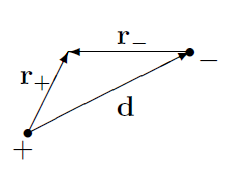
\includegraphics[width=\linewidth]{imagenes/4_IMG.png}
    \label{fig:}
\end{minipage}
\hfill
\begin{minipage}{0.6\textwidth}
    Siendo \textbf{d} vector desde el centro de la positiva al centro de la negativa como se muestra en el gráfico.
\end{minipage}

Finalmente, el campo eléctrico total es
\[
\boxed{\textbf{E} = \frac{\rho}{3 \varepsilon_0} \textbf{d}}
\]



%----------------------------------------------Ej_Michel---------------------------------
%---------------------------------------------Ej_20_IDMCh---------------------------------
\section*{\question{ Problema 2.20}} Uno de estos es un campo electrostático imposible. ¿Cuál?

\begin{enumerate}[label=(\alph*)]
    \item  \(\mathbf{E} = k[xy \mathbf{ \hat{x}}+ 2yz\mathbf{ \hat{y}}+ 3zx\mathbf{ \hat{z}}] \)
    \item \(\mathbf{E} = k[y^2\mathbf{ \hat{x}}+ (2xy + z^2)\mathbf{ \hat{y}}+ 2zx\mathbf{ \hat{z}}] \)
\end{enumerate}

Donde \(k\)  es una constante con las unidades adecuadas. Para el campo posible, encuentre el potencial \(V\), usando el origen como unto de referencia. Verifique su respuesta calculando el \(\nabla V\) y comparando con el campo eléctrico que encontró en el inciso a.(Pista: Debe elegir una trayectoria específica para integrar. La respuesta es independiente de la trayectoria, pero no puede integrar sin definir una.)

\subsection*{Solución:}
Para un campo electrostático, el rotacional del campo eléctrico debe ser cero. Por lo tanto, para determinar si un campo es electrostático o no, debemos calcular el rotacional de cada uno de los campos eléctricos propuestos.

\subsubsection*{Para el campo (a)}

Calculo del rotacional el rotacional:

\[
\nabla \times \mathbf{E} = 
\begin{vmatrix}
\hat{\mathbf{x}} & \hat{\mathbf{y}} & \hat{\mathbf{z}} \\
\partial_x & \partial_y & \partial_z \\
kxy & 2k yz & 3k xz
\end{vmatrix}
\]

\begin{align*}
(\nabla \times \mathbf{E})_x &= \frac{d}{dy} (3kxz) - \frac{d}{dz} (2kyz) = 0 - 2ky = -2ky \\
(\nabla \times \mathbf{E})_y &= \frac{d}{dz} (kxy) - \frac{d}{dx} (3kxz) = 0 - 3kz = -3kz \\
(\nabla \times \mathbf{E})_z &= \frac{d}{dx} (2kyz) - \frac{d}{dy} (kxy) = 0 - kx = -kx
\end{align*}

\[
\nabla \times \mathbf{E} = -2ky\,\hat{\mathbf{x}} - 3kz\,\hat{\mathbf{y}} - kx\,\hat{\mathbf{z}} \neq \mathbf{0}
\]


%--- mod 


\boxed{\text{El campo (a) es imposible}}


\subsubsection*{Para el campo (b)}
Calculamos el rotacional:

\[
\nabla \times \mathbf{E} = 
\begin{vmatrix}
\hat{\mathbf{x}} & \hat{\mathbf{y}} & \hat{\mathbf{z}} \\
\partial_x & \partial_y & \partial_z \\
ky^2 & k(2xy + z^2) & 2kyz
\end{vmatrix}
\]

\begin{align*}
(\nabla \times \mathbf{E})_x &= \frac{d}{dy} (2kyz) - \frac{d}{dz} (kz^2) = 2kz - 2kz = 0 \\
(\nabla \times \mathbf{E})_y &= \frac{d}{dz} (ky^2) - \frac{d}{dx} (2kyz) = 0 - 0 = 0 \\
(\nabla \times \mathbf{E})_z &= \frac{d}{dx} (2kxy) - \frac{d}{dy} (ky^2) = 2ky - 2ky = 0
\end{align*}

\[
\nabla \times \mathbf{E} = \mathbf{0}
\]

\subsection*{Cálculo del potencial para (b)}
Integrando a lo largo de la trayectoria \((0,0,0) \to (x,0,0) \to (x,y,0) \to (x,y,z)\):

\begin{figure}[ht]
    \centering
    \tdplotsetmaincoords{70}{120} % ángulo de vista

    \begin{tikzpicture}[tdplot_main_coords, scale=3]

        % Ejes coordenados
        \draw[->] (0,0,0) -- (1.5,0,0) node[anchor=north east]{$x$};
        \draw[->] (0,0,0) -- (0,1.5,0) node[anchor=north west]{$y$};
        \draw[->] (0,0,0) -- (0,0,1)   node[anchor=south]{$z$};

        % Coordenadas de trayectoria
        \coordinate (a) at (1,0,0);
        \coordinate (b) at (1,1,0);
        \coordinate (c) at (1,1,1); % Este es el punto final

        % Trayectoria en pasos
        \draw[thick, red, ->] (0,0,0) -- (a) node[anchor=south east] {$(x_0)$} node[midway , above] {$\lambda_1$};
        \draw[thick, blue, ->] (a) -- (b) node[anchor=south west] {$(y_0)$} node[midway , above] {$\lambda_2$};
        \draw[thick, green, ->] (b) -- (c) node[anchor=north west] {$(z_0)$} node   [midway , right] {$\lambda_3$};

        % Punto final
        \filldraw[black] (c) circle (0.5pt);
        \node[anchor=south] at (c) {$(x_0, y_0, z_0)$};

    \end{tikzpicture}
    \caption{Trayectoria $(x_0, y_0, z_0)$}
\end{figure}




Parametrizando  la trayectoria con respecto a un parametro \(t\) 
\[ \lambda = \lambda_1 + \lambda_2 + \lambda_3\]
\[
\lambda[0, r_0]: \longrightarrow  \mathbf{R^3}   
\]
% preguntar al profe por la notación de la trayectoria
\[ \lambda_1 = (t,0,0),\, \lambda_1' = (1,0,0)dt \]
\[ \lambda_2 = (0,t,0),\, \lambda_2' = (0,1,0)dt \]
\[ \lambda_3 = (0,0,t),\, \lambda_3' = (0,0,1)dt \]
\[
V(x,y,z) = -\int_0^{x_0} \mathbf{E}\cdot d \lambda_1' -\int_0^{y_o} \mathbf{E}\cdot d \lambda_2'-\int_0^{z_0} \mathbf{E}\cdot d \lambda_3'
\]
Trayectoria \(\lambda_1\): \((0,0,0) \to (x_0,0,0)\)
\begin{align*}
    \int_0^{x_0} \mathbf{E}\cdot d \lambda_1'& =  \int_0^x k((0)^2,[2(t)(0) + 0^2],2(0)) \cdot (1,0,0)dt\\
& = 0
\end{align*}
Trayectoria \(\lambda_2\): \((x_0,0,0) \to (x_0,y_0,0)\)
\begin{align*}
    \int_0^{y_0} \mathbf{E}\cdot d \lambda_2'& =  \int_0^{y_0} k((t)^2,[2(x_o)(t) + 0^2],2(0)(t)) \cdot (0,1,0)dt\\
& = \int_0^{y_0} k((t)^2,[2(x_0)(1) + 0^2],2(0)(t)) \cdot (0,1,0)dt\\
& = \int_0^{y_0} 2kx_o t dt\\
& = kx_0 t^2 \bigg|_0^{y_0} \\
& = kx_0 y_0^2
\end{align*}
Trayectoria \(\lambda_3\): \((x_0,y_0,0) \to (x_0,y_0,z_0)\) 
\begin{align*}
    \int_0^{z_0} \mathbf{E}\cdot d \lambda_2'& =  \int_0^{z_0} k((yo)^2,[2(x_o)(y_0) + t^2],2(t)(y_0)) \cdot (0,0,1)dt\\
& = \int_0^{z_0} k((y_0)^2,[2(x_0)(y_0) + t^2],2(t)(y_0)) \cdot (0,0,1)dt\\
& = \int_0^{z_0} 2ky_o t dt\\
& = ky_0 t^2 \bigg|_0^{z_0} \\
& = ky_0 z_0^2
\end{align*}

\begin{align*}
    V(x,y,z)& = -kx_0 y_0^2 - ky_0 z_0^2\\
& =-k[x_0y_0^2 + y_0z_0^2] \\
\end{align*}
En general 
\[\boxed{ V(x,y,z) = -k(xy^2 + yz^2)}\]


Verificación, calculando el Gradiente del potencial:
\begin{align*}
    \mathbf{ \nabla}V & = \frac{\partial V}{\partial x} \hat{\mathbf{x} } + \frac{\partial V}{\partial y}  \hat{\mathbf{y} } + \frac{\partial V}{\partial z}  \hat{\mathbf{z} }\\
    \mathbf{ \nabla }V & = -k(y^2)\hat{\mathbf{x} } -k(2xy + z^2)\hat{\mathbf{y} } -k(2yz)\hat{\mathbf{z} } \\
    \mathbf{ \nabla }V  & = -k\left(y^2\,\hat{\mathbf{x}} + (2xy + z^2)\,\hat{\mathbf{y}} + 2yz\,\hat{\mathbf{z}}\right) 
\end{align*}

\[
    \boxed{V(x,y,z) = -k(xy^2 + yz^2)}
\]


%--------------------------------------------Ej_22_IDMCh---------------------------------
\section*{\question{ Problema 2.22}} Hallar el potencial eléctrico V a una distancia s de un alambre recto infinitamente largo que transporta una carga lineal uniforme \(\lambda\)

\subsection*{Solución:}
Para encontrar el potencial \(V\) de un campo eléctrico dado,  usamos la integral de línea del campo eléctrico sobre una trayectoria que va desde el punto \((0,0,0)\) hasta el punto \((x,y,z)\)
\[
{V(s)} = -\int_{r_o}^{\mathbf{r}} \mathbf{E}\cdot d \mathbf{l}   
\]    

para un alambre recto infinitamente largo, el campo eléctrico es radial y tiene la forma:
\[
\mathbf{E} = \frac{\lambda}{2\pi \epsilon_0 s} \hat{\mathbf{s}}
\]

Reemplazando en la integral de línea, tenemos:
\[
    {V(s)} = -\int_{s_o}^{s} \frac{\lambda}{2\pi \epsilon_0 s} ds 
\]
\[
\boxed{{V(s)} =  -\frac{\lambda}{2\pi \epsilon_0} \ln{\frac{s}{s_o} }}
\]

Para comprobar el resultado, calculamos el campo eléctrico a partir del potencial:
Además, dado que el sistema esta en coordenadas cilíndricas el campo eléctrico se puede calcular como:

\begin{align*}
    \mathbf{E}  &= -\nabla V = -\frac{\partial V}{\partial s} \hat{s} \\
    \mathbf{E} &= -\frac{\partial}{\partial s} \left(-\frac{\lambda}{2\pi \epsilon_0} \ln{\frac{s}{s_o} } \right) \\
    \mathbf{E} &= \frac{\lambda}{2\pi \epsilon_0} \frac{1}{s} \hat{\mathbf{s}} \\
\end{align*}
\[
\boxed{\mathbf{E} = \frac{\lambda}{2\pi \epsilon_0 s} \hat{\mathbf{s}}}
\]
%---------------------------------------------Ej_24_IDMCh---------------------------------

\section*{\question{ Problema 2.24}}Para la configuración del problema 2.16, calcule la diferencia de potencial entre un punto en el eje y un punto en el cilindro exterior. Observe que no es necesario elegir un punto de referencia específico si se utiliza la ecuación 2.22.
\subsection*{Solución:}
\tdplotsetmaincoords{70}{120}

\begin{figure}[H]
    \centering
    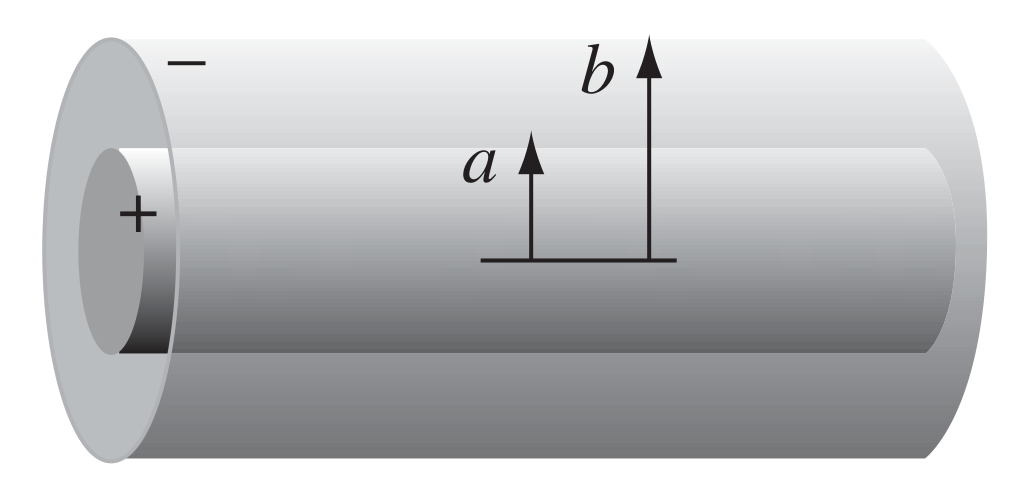
\includegraphics[width=0.5\textwidth]{imagenes/problema_24.png}
    \caption{\label{fig:problema_24}Configuración del problema 2.16}
\end{figure}


Del Problema 2.16 tenemos que el campo eléctrico es:
\begin{enumerate}[label=(\roman*)]
    \item Para \(0 < s < a\) tenemos:
        \[
        \mathbf{E} = \frac{\rho s}{2\epsilon_o }  \hat{s}
        \]
    \item  para \( a < s < b \) tenemos:
            
        \[
        \mathbf{E} = \frac{\rho a^2}{2\epsilon_o s }  \hat{s}
        \]
\end{enumerate} 

% insertar figura del campo eléctrico
La diferencia de potencial entre un punto en el eje y un punto en el cilindro exterior es:
\[
{V(b)}-{V(0)}   = -\int_{0}^{b} \mathbf{E}\cdot d \mathbf{l}  
\]
Dado el intervalo de integración se puede separar la integral en dos partes:

Desde  \(a < s < b\) y  \(0 < s <a\)
\begin{align*}
    {V(b)}-{V(0)}   &= -\int_{a}^{b} \frac{\rho a^2}{2\epsilon_o s } ds - \int_{0}^{a} \frac{\rho s}{2\epsilon_o } ds \\
    &= -\left[\frac{\rho a^2}{2\epsilon_o} \ln(s) \right]_{a}^{b} - \left[\frac{\rho s^2}{4\epsilon_o} \right]_{0}^{a} \\
    &= -\frac{\rho a^2}{2\epsilon_o} \left[\ln(b) -\ln(a)  \right] - \left[\frac{\rho a^2}{4\epsilon_o} + 0 \right] \\
    &= -\left[\frac{\rho a^2}{2\epsilon_o} \ln{\frac{b}{a} } \right] - \left[\frac{\rho a^2}{4\epsilon_o} \right] \\
    &= -\frac{\rho a^2}{2\epsilon_o} \ln{\frac{b}{a} } - \frac{\rho a^2}{4\epsilon_o}\\
\end{align*}
\[
\boxed{V(b)-V(0) =-\frac{\rho a^2}{4\epsilon_o} \left(2\ln{\frac{b}{a} } + 1 \right) }
\]
\end{document}